
\documentclass{article}
%%%%%%%%%%%%%%%%%%%%%%%%%%%%%%%%%%%%%%%%%%%%%%%%%%%%%%%%%%%%%%%%%%%%%%%%%%%%%%%%%%%%%%%%%%%%%%%%%%%%%%%%%%%%%%%%%%%%%%%%%%%%%%%%%%%%%%%%%%%%%%%%%%%%%%%%%%%%%%%%%%%%%%%%%%%%%%%%%%%%%%%%%%%%%%%%%%%%%%%%%%%%%%%%%%%%%%%%%%%%%%%%%%%%%%%%%%%%%%%%%%%%%%%%%%%%
\usepackage{geometry}
\usepackage{fancyhdr}
\usepackage[pdftex]{graphicx}

%TCIDATA{OutputFilter=LATEX.DLL}
%TCIDATA{Version=5.50.0.2953}
%TCIDATA{<META NAME="SaveForMode" CONTENT="1">}
%TCIDATA{BibliographyScheme=Manual}
%TCIDATA{Created=Monday, January 30, 2012 17:20:46}
%TCIDATA{LastRevised=Monday, February 27, 2012 12:06:08}
%TCIDATA{<META NAME="GraphicsSave" CONTENT="32">}
%TCIDATA{<META NAME="DocumentShell" CONTENT="Standard LaTeX\Blank - Standard LaTeX Article">}
%TCIDATA{CSTFile=40 LaTeX article.cst}

\newtheorem{theorem}{Theorem}
\newtheorem{acknowledgement}[theorem]{Acknowledgement}
\newtheorem{algorithm}[theorem]{Algorithm}
\newtheorem{axiom}[theorem]{Axiom}
\newtheorem{case}[theorem]{Case}
\newtheorem{claim}[theorem]{Claim}
\newtheorem{conclusion}[theorem]{Conclusion}
\newtheorem{condition}[theorem]{Condition}
\newtheorem{conjecture}[theorem]{Conjecture}
\newtheorem{corollary}[theorem]{Corollary}
\newtheorem{criterion}[theorem]{Criterion}
\newtheorem{definition}[theorem]{Definition}
\newtheorem{example}[theorem]{Example}
\newtheorem{exercise}[theorem]{Exercise}
\newtheorem{lemma}[theorem]{Lemma}
\newtheorem{notation}[theorem]{Notation}
\newtheorem{problem}[theorem]{Problem}
\newtheorem{proposition}[theorem]{Proposition}
\newtheorem{remark}[theorem]{Remark}
\newtheorem{solution}[theorem]{Solution}
\newtheorem{summary}[theorem]{Summary}
\newenvironment{proof}[1][Proof]{\noindent\textbf{#1.} }{\ \rule{0.5em}{0.5em}}
% Sets page margins to 1", which is standard
\geometry{left=1in,right=1in,top=1in,bottom=1in} 
% allows the included extensions of graphic files
\DeclareGraphicsExtensions{.pdf,.png,.jpg}
% sets graphic path. Otherwise it just looks around
\graphicspath{{}}
% I do not remember what this does
\setlength{\headheight}{15.2pt}
% allows the xhead parameters
\pagestyle{fancy}
% replace with your name
\lhead{Group \#10}
% replace 
\rhead{Group 10 IS BEST GROUP}
% \input{tcilatex}
\begin{document}

% INCLUDEGRAPHICS EXPLANATION
% \includegraphics[scale=1]{name of file}
% sometimes you want to twice encase the filename in squiggly brackets. I do not know why but sometimes it is required.

% begin title page, use \\ for newline
\title{\#EEDS\\Report from Lab Assignment \#1\\TDT4258 Energy Efficient Computer Systems}
% now one can list the authors, \textbf{} makes bold text
\author{Emil Taylor Bye}
\author{Sigve Sebastian Farstad}
\author{Odd M. Trondrud}
% make title page
\maketitle

% create new page
\newpage

% uncomment this if you want to include a ToC
% \tableofcontents
% disables chapter, section and subsection numbering
% set to 1 or higher to enable section numbering
% it goes something like 0:Part, 1:Section, 2:Section, 3:Subsection, 4:Subsubsection, ...
\setcounter{secnumdepth}{-1}

% use \newpage to get newpage
% \bigskip to get some space between paragraphs
% \texttt{TEXTHERE} to get typewriter-like (basically just monospaced) text

\part{Abstract}

This report is the solution to assignment 1 of TDT4258 at NTNU, spring 2013.
In the assigment, an Atmel STK1000 development board is programmed to display a moveable LED 'paddle' using AVR32 assembly and the GNU tool chain.

\part{Introduction}

This report presents a solution to assignment \#2 of TDT4258 at NTNU, during the spring of 2013.
The objective of this lab assignment is to write a program in C for the STK1000 development board which causes different sounds to play when different buttons on the board are pressed, using an interrupt routine to pass the audio samples to the board's ABDAC (Audio Bitstream Digital to Analog Converter).
A minimum of three different sound effects should be made, as well as a ``start up melody''.

This report details the development of the sound-generating program as a solution to the assignment.
\section{The STK1000}
	The STK1000 is a development board from Atmel which offers a complete development environment for Atmel's AT32AP7000 processor.
	It offers a multitude of different peripheral I/O devices, of which this assignment will be using an array of LEDs and some push buttons.
	The processor is an ARM32 processor, and will for this assignment be only running the assembled output of hand-coded C code, without the support of an operating system.

\section{A note on sound}
	In order to write a program to generate sound, one should first study the physical properties of sound, and research different strategies to generate sound in a digital environment.

Sound is a mechanical wave that is an oscillation of pressure composed of frequencies within the range of hearing\footnote{http://en.wikipedia.org/wiki/Sound}.

Humans can percieve sounds with frequencies that range from about 20Hz - the lowest of basses - to 20kHz - the highest of high-pitched whining.
Sound is inherently analog, and requires some form of digital representation to be able to be generated by the AP7000, which is a digital device.
Regarding a sound wave as a continuous signal representing wave amplitude with respect to time, one straight-forward way of representing a sound wave digitally is to simply have an list of integer signal samples at a fixed, preferrably small, time interval.
This is indeed the format the AP7000 expects for its digital-to-analog converter.

There are different strategies available for preparing the stream of integers that needs to be sent to the digital-to-analog converter to generate a sound.
One strategy is simply to store the prepared list of integers somewhere in memory, and then copy it over to the DAC integer by integer as they are consumed by the ABDAC.
This strategy is analogous to rasterized bit maps in the image world.
This strategy, while easy to implement, and is able to represent all kinds of sounds, requires a great deal of memory (integer size * sample rate of bytes per second, in fact).
As an example, a three minute song, when stored at 16 bits per sample at a generously low sample rate of 22050Hz, requires 16 bits/sample * 180 seconds * 22050 samples/second = ̃ca 7.57 megabytes.
To put this in perspective, the entire flash memory of the AP7000 is 8 megabytes.
On a low memory platform like the STK1000, this is therefore not a great strategy.

Another strategy is the generative approach.
This strategy is analogous to vector based images in the image world.
The idea is to generate samples at run-time based on configurations read from memory, rather than reading the pre-generated values from memory.
This is a more CPU-hungry approach, but requires less memory than the previous strategy.
This strategy is used for the sound effect synth in the presented solution program.

A third strategy is a hybrid approach, where small sample lists are pre-bundled with the program, and generative rules are used to play back the samples at different times with different parameters.
This is the approach used in the music player in the presented solution program.



\section{About the MOD file format}
	The MOD file format is an old music tracker file format originally created for the Commodore Amiga (figure \ref{img-amiga}), a series of computers from the late eighties.
\begin{figure}[H]
	\caption{The Amiga 1000 (1985), the first Amiga model released. Image courtesy of Kaiiv.}
	\centering
	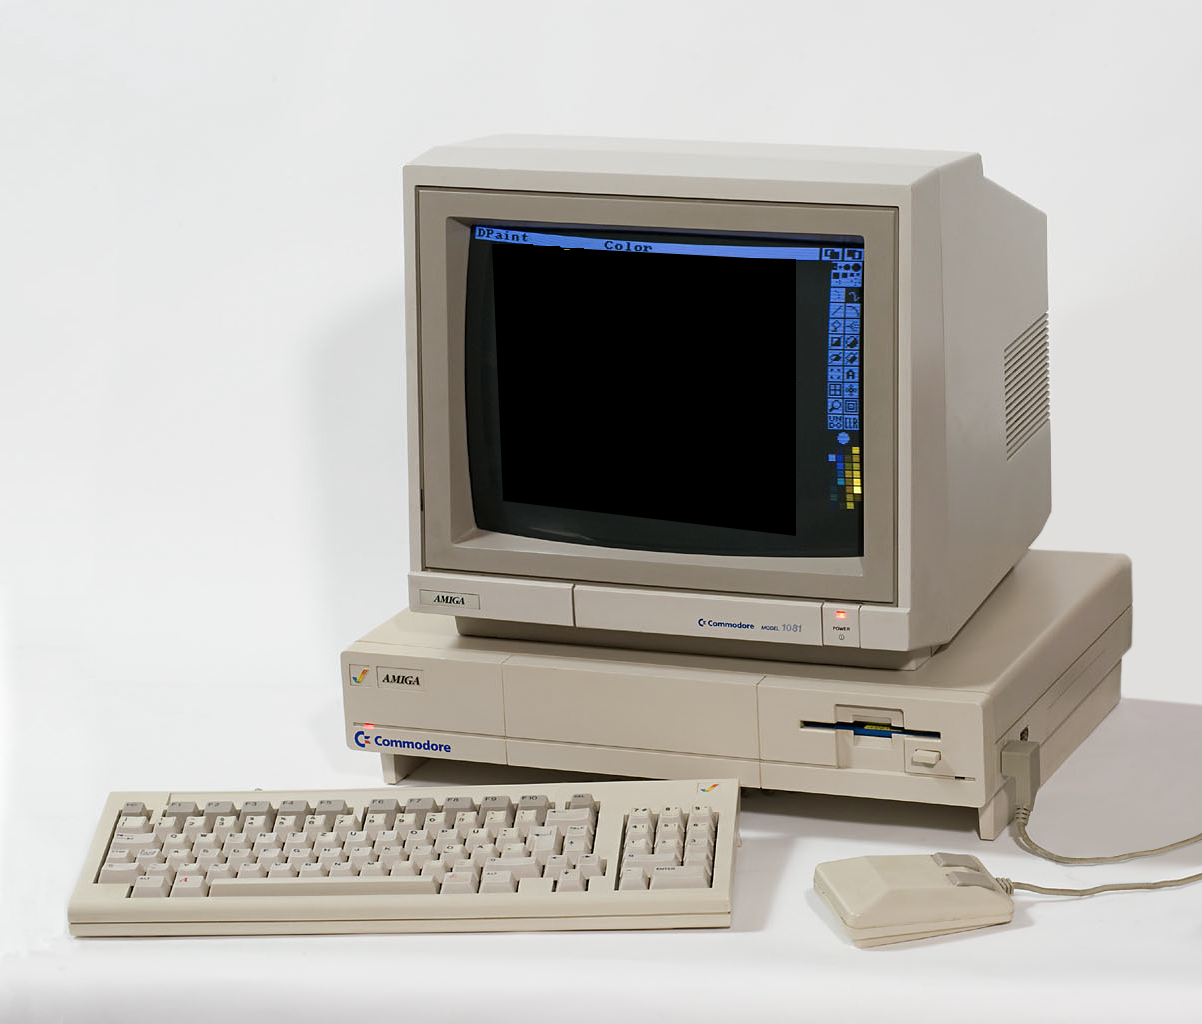
\includegraphics[width=4in]{{images/Amiga.jpg}}
    \label{img-amiga}
\end{figure}

The file format is tightly optimized for playback on the Amiga's audio hardware, so to understand the inner workings of the MOD file format, one should first know a little about how the Amiga's audio hardware works.

The Amiga's sound chip, called Paula, is capable of powering four simultaneous DMA-driven 8-bit PCM sample sound channels.
Each of these channels can be independently set to different sample frequencies many times per second.
The MOD format exploits this -- it supports 4 simultaneous channels of sample playback, using the frequency modulation to change the pitch of the samples played in the different channels.

Internally, the music in a MOD file is stored as a set of PCM-coded predefined sounds, as well as a large table of note patterns containing information about which sounds should be played at which frequencies and at which time.
The MOD format also includes a large set of musical effects such as tremolo, vibrato, arpeggio, portamento and so on, a subset of which are implemented in the presented solution program.

The MOD file format is not a defined standard, and does therefore not have a formal specification.
The MOD format grew organically from the early Amiga demoscene in the eighties, so many different variants exist -- each with with their own specialities and quirks.
The MOD Player presented in the solution is tailored to read so-called \texttt{M.K.} MODs generated by a MOD creator program (``tracker'') called ProTracker.
These MOD files are called \texttt{M.K.} MODs because they contain the magic number \texttt{M.K.} in the file header.
This is one of the most popular MOD formats, and has become a sort informal standard amongst MOD trackers.

\texttt{M.K.} MODs can have a maximum of 31 bundled PCM-coded sounds, 128 patterns, each with 64 note divisions for each of the four channels, and a a 128 item long list of which patterns should be played in what order.

Figure \ref{img-protracker} shows an image of a MOD file being edited in a tracker program.
Each column represents one channel, and each row represents one of the 64 divisions of a pattern.
The currently played division is traditionally kept vertically centered in the middle of the screen, as in this image.


\begin{figure}[H]
	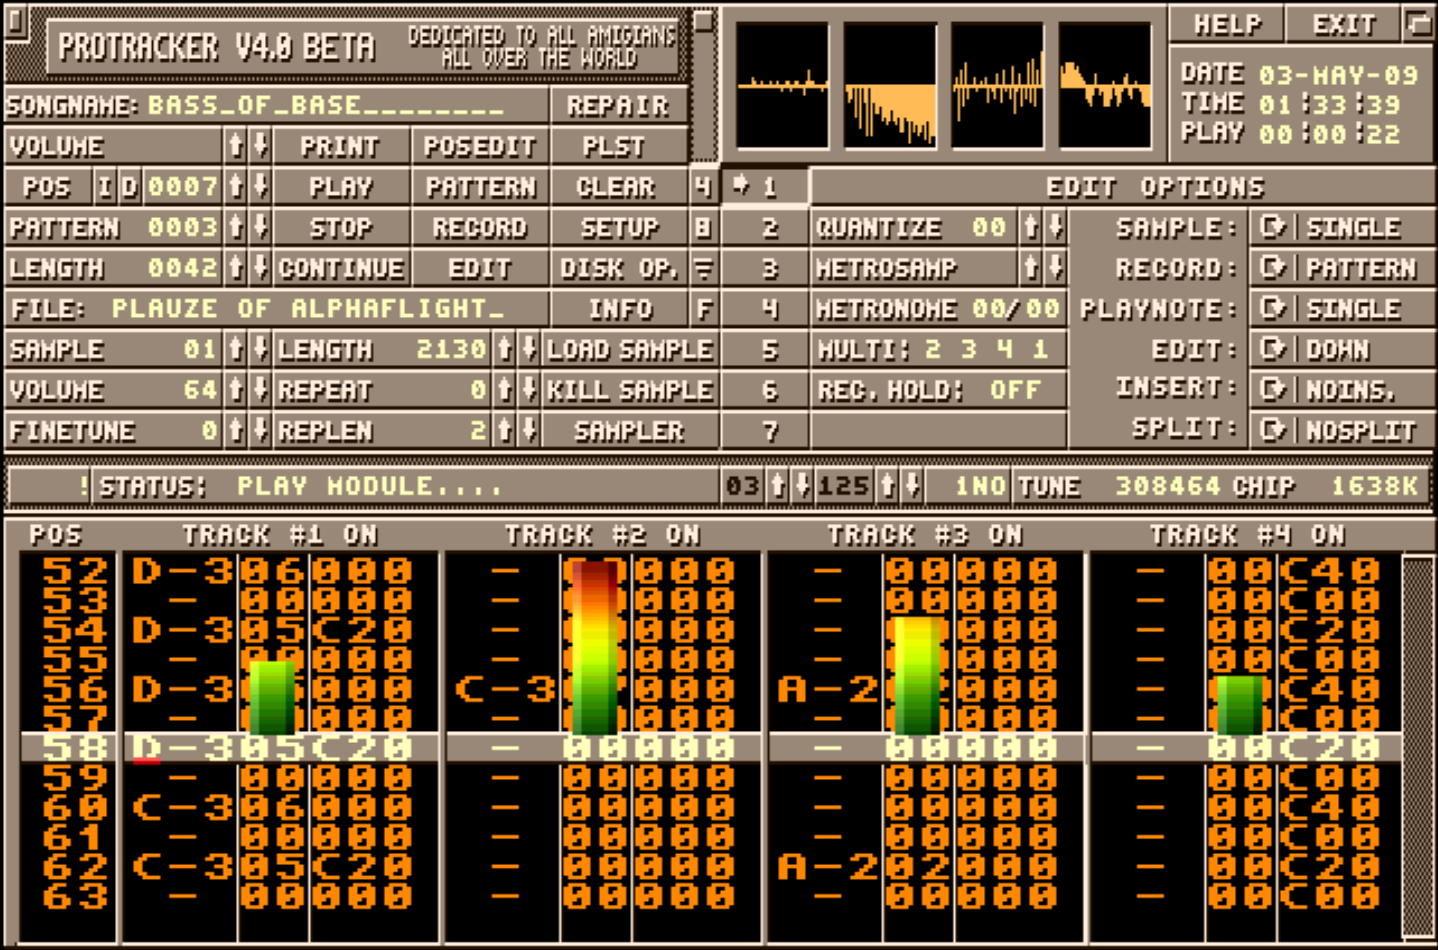
\includegraphics[width = \textwidth]{images/Protracker.png}
	\caption{A four-channel MOD being played in ProTracker. Image courtesy of Alec Graggamoor.}
	\label{img-protracker}
\end{figure}

These four resources do a pretty good job of documenting the MOD file format in detail:
\begin{itemize}
	\item{\url{http://www.mediatel.lu/workshop/audio/fileformat/h_mod.html}}
	\item{\url{http://archive.cs.uu.nl/pub/MIDI/DOC/MOD-info}}
	\item{\url{https://bel.fi/alankila/modguide/}}
	\item{\url{http://16-bits.org/mod/}}
\end{itemize}

\newpage


\part{Description and Methodology}

This is the description and methodology.

\subsection{Configuration of the STK1000}

\subsubsection{Jumpers}

The STK1000 has 10 jumpers that can be set to configure the board.
For this assignment the jumpers were set as specified on page 37 in \cite{lab-compendium}.


\subsubsection{GPIO connections}

The STK1000 provides a general purpose input/output interface (\texttt{GPIO}) with 32 signal lines.
16 of the 32 available lines were connected to on-board I/O devices on the STK1000 in this assignment.
The I/O devices in use were 8 on-board LEDs, used as a rudimentary paddle display, and 8 on-board switches, used as player controls.

The buttons were connected to \texttt{GPIO0-GPIO7} (\texttt{J1} on the STK1000) using a flat cable as in figure \ref{flat-cable-image}. This maps the buttons to ports \texttt{0-7} of \texttt{PIOB}.
The choice of low port numbers \texttt{0-7} is convenient for coding, and the choice of \texttt{PIOB} as opposed to \texttt{PIOC} is purely mnemonic ('B' for buttons).

The LEDs were connected to \texttt{GPIO16-GPIO23} (\texttt{J3} on the STK1000) using a flat cable as in figure \ref{flat-cable-image}. This maps the LEDs to ports \texttt{0-7} of \texttt{PIOC}.
Having the same port numbers for the buttons and the LEDs is a nice convenience for cleaner and more efficient code, as translation from button ports to LED ports is not necessary.

\begin{figure}
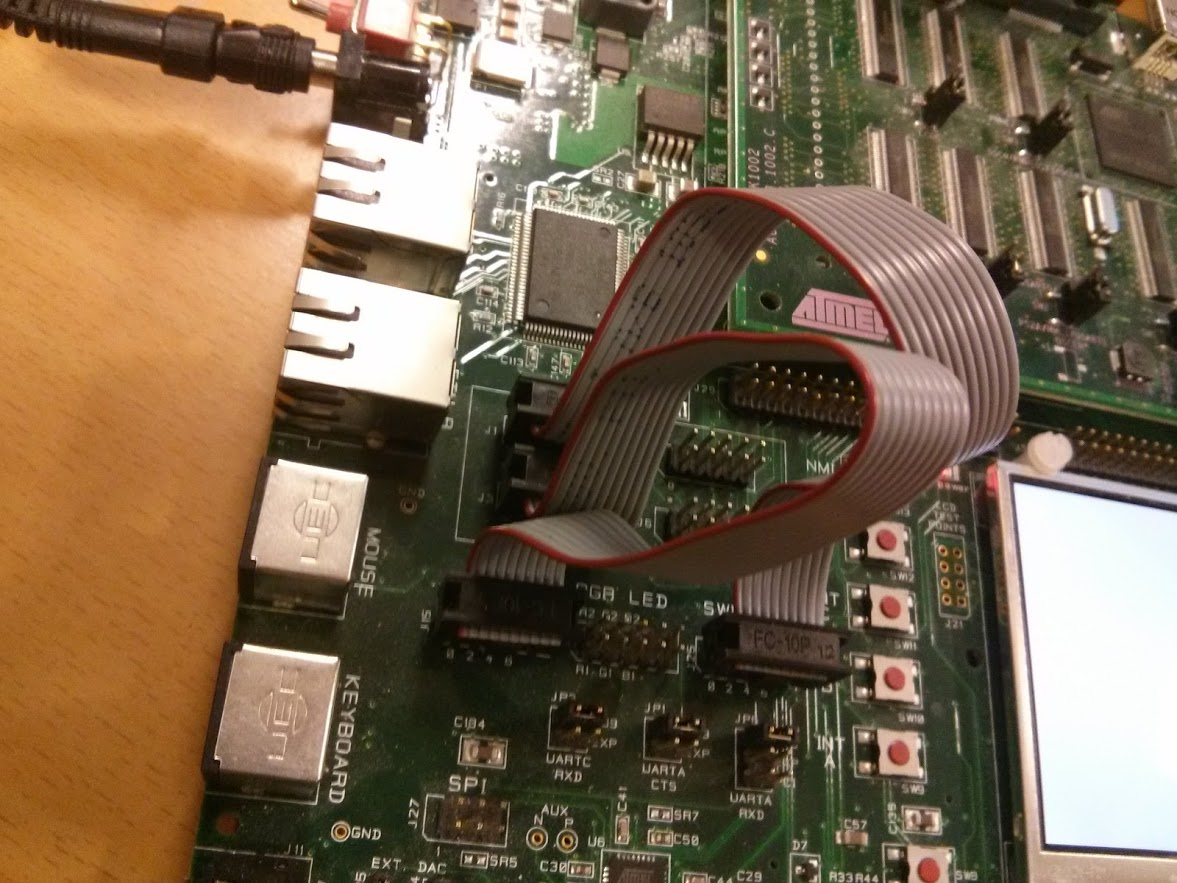
\includegraphics[width = \textwidth]{description-and-methodology/flat-cable-image.jpg}
\caption{Flat cables connecting GPIO with switches and LEDs. Note the orientation of the flat cables.}
\label{flat-cable-image}
\end{figure}


\subsection{Programming environment}

\subsubsection{JTAGICE}

<General info about JTAGICE>.
The JTAGICE was connected to the STK1000 (taking care not to connect the connector upside-down) and the PC using <cables>.

\subsubsection{GNU Debugger}

\subsubsection{Make, other tools etc}

\subsection{Development of the program}

\subsubsection{Setting up the LED diodes}

\subsubsection{Setting up the buttons}

\subsubsection{Interrupt Routine}

\subsubsection{Refactoring and Modularization}

\subsubsection{Register Overview}

<description of which registers do what>

\subsubsection{Program flow}

<diagrams, descriptions>

yuml.me-source for diagrams

Main program flow:
(start)->(Init)->(Main loop)->(Main loop)


Init:
(start)->(Load pointers)->(Set up start values in registers)->(Enable I/O with interrupts)->(end)

Main loop:
(start)->(Set leds)->(Sleep)[interrupt]-><interrupt routine>->[Was SW0 pressed][Yes]->(Move paddle right)->(end),[Was SW0 pressed][No]->(Move paddle left)->(end)


Set leds:
(start)->(Turn off all LEDs)->(Turn on the paddle LED)->(end)

Button interrupt routine:
(start)->(Read button states)->(Software debounce)->(Notify that the interrupt has been handled)->(end)

Debounce:
(start)->(Set register to a high constant)->(Is value in register equal to 0)[Yes]->(end),(Is value in register equal to 0)[No]->(Decrease value in register by 1)->(Is value in register equal to 0)

Read buttons:
(start)->(Read button status)->(Mask away buttons that were pressed in previous interrupt)->(end)

Move paddle right:
(start)->(Is paddle at far-right end of the board)[Yes]->(Move paddle to far-left)->(end),(Is paddle at far-right end of the board)[No]->(Move paddle one step to the left)->(end)

Move paddle left (analogous to move paddle right, but included for completeness):
(start)->(Is paddle at far-left end of the board)[Yes]->(Move paddle to far-right)->(end),(Is paddle at far-left end of the board)[No]->(Move paddle one step to the right)->(end)



\part{Results and Tests}

This is the results and tests section.

\subsection{Energy Efficiency}

\subsection{Testing}

\part{Evaluation of Assignment}

Here comes the evaluation of the assignment.

\part{Conclusion}

This is the place for the conclusion.

\part{Acknowledgement}

Here, we acknowledge those who deserve to be acknowledged.

\part{References}

And finally, references.

\end{document}
